\documentclass[11pt,a4paper]{article}
\usepackage[margin=24mm]{geometry}\usepackage{fontspec,unicode-math,booktabs,graphicx,hyperref}
\setmainfont{STIXGeneral}\setmathfont{STIX Two Math}
\title{Odd kernels and cyclotomic constructions\\Complete manuscripts and optional validation}
\author{Human Compression project}\date{}
\begin{document}\maketitle
Two complete originals are compared with one common paper and two complete
applications: Hou--Feng--Leemans--Qu, \emph{String C-groups of order $4p^m$}
(L014, arXiv:2407.10388v1, 12 pages), and Kong--Feng--Hou--Leemans--Qu,
\emph{Chiral 3-polytopes of order $2p^m$} (L007, accepted manuscript dated
19 January 2026, 22 pages). The common manuscript retains its title
\emph{Odd kernels, cyclotomic modules and cyclic carries}.

\paragraph{The complete written comparison.}
The primary coordinate, fixed before counting, is raw untrimmed extraction
in NFC, counting characters without whitespace:
\[
 R=\frac{25574+44251}{15876+11504+15894}
 =\frac{69825}{43274}=\mathbf{1.613555}.
\]
It pays the entire common paper once and both applications in full,
including references and scope qualifications. No inherited common proof or
application is free. Optional validation programs are excluded on both sides.
A bounded exact-source audit, reusing the prior complete source and proof
reading, found no executable validation listings in either original or in
these three replacement papers. No text cut is therefore needed.
\begin{center}\begin{tabular}{lrr}\toprule
Complete document&Pages&Characters\\\midrule
Original L014&12&25574\\
Original L007&22&44251\\
Common theory $U$&7&15876\\
Regular application $A_1$&5&11504\\
Chiral application $A_2$&6&15894\\\bottomrule
\end{tabular}\end{center}
\paragraph{Each matched result after common acquisition.}
After acquiring \emph{the entire common theory and the actual retained
mathematical premises}, the local comparisons are
\[
 r_{014}=\frac{25574}{11504}=2.223053,
 \qquad r_{007}=\frac{44251}{15894}=2.784132.
\]
These are conditional application figures, not standalone whole-topic factors.
The measured common cost is 15876; full costs of retained outside proofs remain
unknown. The nine validation programs are optional checks, not prerequisites
of the uniform proofs or these written comparisons.

\paragraph{Whole validation inventory, with no asymmetric ratio.}
All nine files, including two exploratory scans, remain recorded in full:
22466 characters in the nine-page appendix or 21691 in the raw files
(25,501 literal bytes). These are alternative representations, never added
together. Original software costs are unrecorded, not zero; a symmetric
software-inclusive factor is therefore unavailable. The predecessor's
60 one-sided software fractions are withdrawn as compression measures.
\newpage
\begin{center}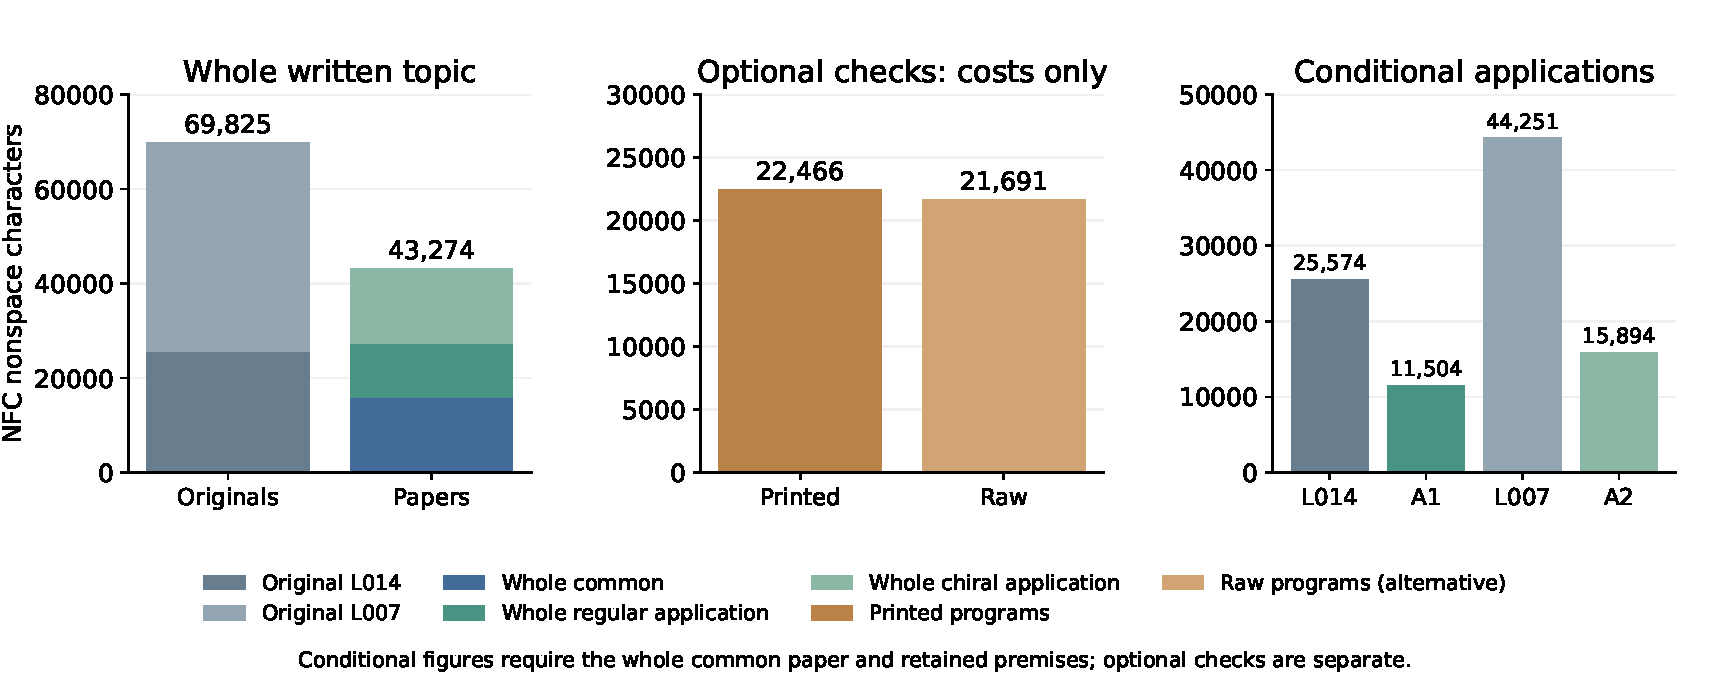
\includegraphics[width=\textwidth]{costs.pdf}\end{center}
\begin{center}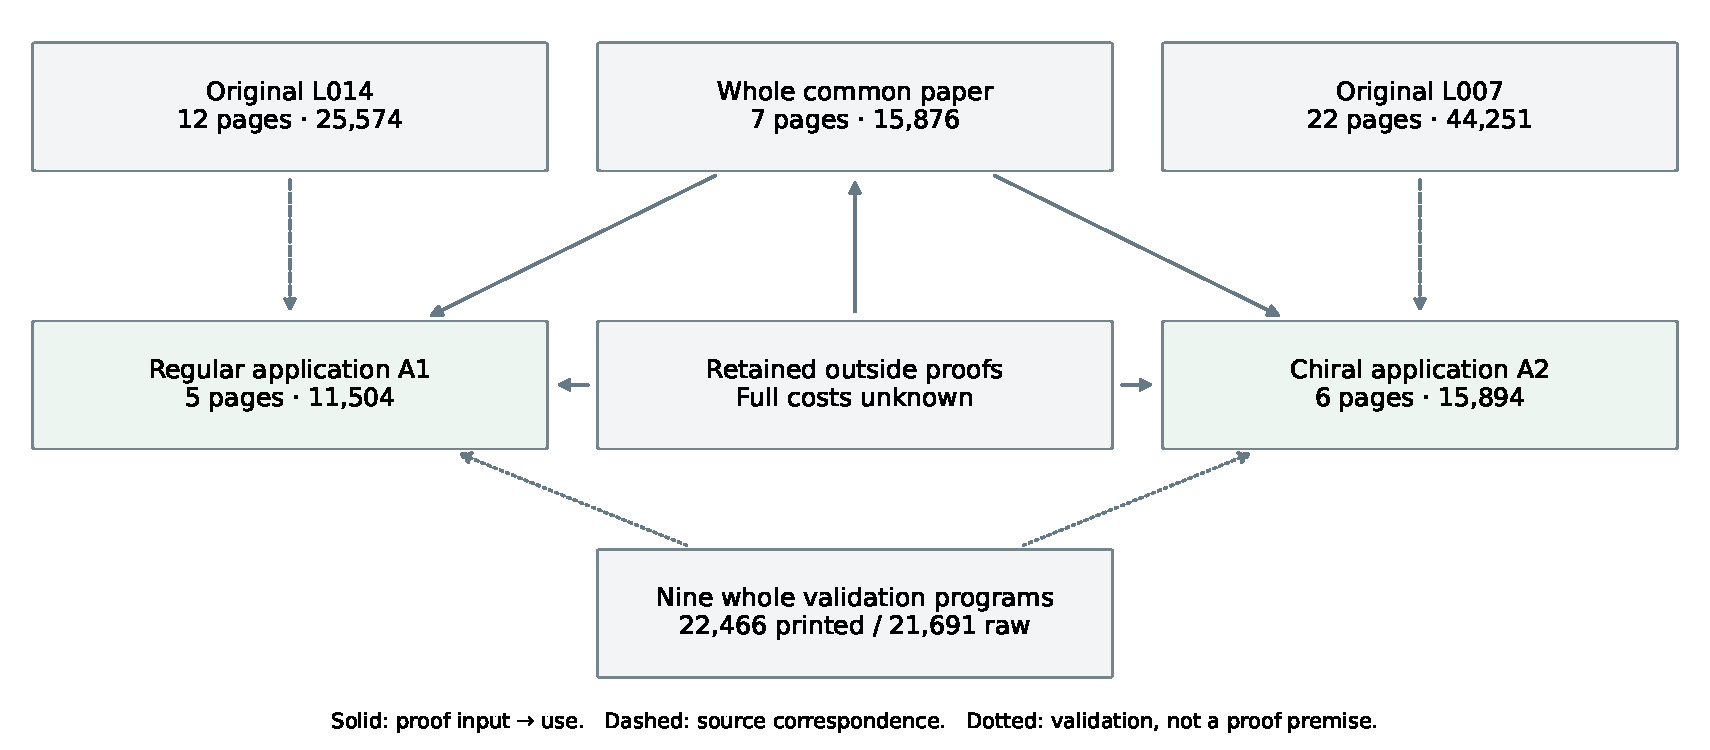
\includegraphics[width=\textwidth]{document_graph.pdf}\end{center}
The graph records whole-document acquisition, not a theorem dependency DAG.
Solid arrows indicate a proof input; dashed arrows match an original to its
application. Dotted arrows associate optional validation with an application.
They do not turn checks into mathematical premises. Every document includes
its local context and references; no node-count factor is inferred.

Acquiring $U$, then all of $A_1$, then all of $A_2$ costs cumulatively
15876, 27380 and 43274 characters. Optional validation may be acquired separately
in either complete representation. Its cost is not included in this written
route or used to inflate conditional prepayment. External proof costs remain
unknown.
\newpage
\paragraph{Unchanged values and unit sensitivities.}
All thirty coordinates and ninety exact fractions are supplied in JSON/CSV:
five units, NFC and NFKC, and raw untrimmed, raw furniture-selected and
calibrated selected text. Every document and raw-file cost and all thirty
written plus sixty conditional fractions equal the immutable predecessor.
Only the comparison policy, acquisition labels and presentation changed.
For untrimmed NFC:
\begin{center}\small\begin{tabular}{lrrr}\toprule
Unit&Whole written&L014 conditional&L007 conditional\\\midrule
Whitespace tokens & 1.918 & 3.186 & 3.051 \\
Alphanumeric units & 1.922 & 2.934 & 3.197 \\
Nonspace characters & 1.614 & 2.223 & 2.784 \\
Collapsed-space characters & 1.673 & 2.397 & 2.837 \\
Collapsed-space UTF-8 bytes & 1.521 & 2.282 & 2.597 \\
\bottomrule\end{tabular}\end{center}
Nonspace-character sensitivities are:
\begin{center}\small\begin{tabular}{llrrr}\toprule
Text&Form&Whole written&L014 conditional&L007 conditional\\\midrule
Untrimmed & NFC & 1.614 & 2.223 & 2.784 \\
Untrimmed & NFKC & 1.614 & 2.227 & 2.783 \\
Selected & NFC & 1.580 & 2.184 & 2.721 \\
Selected & NFKC & 1.581 & 2.188 & 2.720 \\
Calibrated & NFC & 1.580 & 2.184 & 2.721 \\
Calibrated & NFKC & 1.581 & 2.188 & 2.720 \\
\bottomrule\end{tabular}\end{center}
The old one-original report used selected text, costing L014 at 25,115
characters. Its unchanged raw cost is 25,574 and is primary here. That
primary was fixed before the expanded counts. No difference between text
coordinates is a proof saving. Primary text remains literal; selected variants
remove only specified furniture, and font aliases apply only in the calibrated
sensitivity. Complete graphics and formula-layout complexity remain unknown.

\paragraph{Other files and exact scientific scope.}
Four whole operational drivers remain separate: 33,222 bytes (29801
characters). Three complete Lean files are also separate: 9,398 bytes
(6997 characters). Their twelve scoped declarations comprise nine reused
and three new generic statements. They do not formalize the source instances,
complete constructions or geometric correspondence.

All 25 L014 clauses and 38 L007 dispositions are preserved: the marking
correction, every odd/even parameter range, the orientation bridge, the
Section 6 quotient repair, and the fourth regular family in L007 Remark 1.3,
which exists exactly at $p=3$. The inherited cyclic lift has a distinct fresh
root adjudication and is included in $U$.

The Cunningham--Pellicer classification retains its acquired-source
qualification. Huppert, Schmidt--Iwasawa and the declared classical group,
cyclotomic and polytope facts remain premises. Their full proof costs,
source software, runtime and operational engineering are unknown, not zero.
Written length is not complete executable-proof cost or minimal proof
complexity. Scientific/input acceptances are reused; this additive arithmetic
requires distinct review. Its author also authored the predecessor and the
bounded policy audit; no independent numerical acceptance is claimed here.
No source, question, formal or priority credit is assigned by this report.
\end{document}
